% !TeX program = xelatex
\documentclass[lang=cn,a4paper,newtx,bibend=biber]{elegantpaper}
\usepackage[x11names]{xcolor}
\usepackage{tikz}
\usepackage{float}
\usepackage{booktabs}
\usepackage{enumitem}
\usepackage[capitalise,noabbrev]{cleveref}
\usetikzlibrary{arrows.meta,calc,positioning}

\title{AVL Tree Implementation and Evaluation}
\author{Yixiang Chen \and Renhui Lin}
\date{Advanced Data Structures \textbar\ Fall--Winter 2026}
\addbibresource[location=local]{reference.bib}

\definecolor{avlblue}{HTML}{1F4E79}
\definecolor{avlgreen}{HTML}{2F7D6D}
\definecolor{avlorange}{HTML}{D97706}
\colorlet{lightblue}{avlblue!8}
\newcommand{\code}[1]{\texttt{#1}}
\newcommand{\bfactor}[1]{\ensuremath{\mathrm{BF}(#1)}}
\lstset{language=C++,basicstyle=\small\ttfamily,keywordstyle=\color{avlblue}\bfseries,
  commentstyle=\color{avlgreen},stringstyle=\color{avlorange},
  frame=single,rulecolor=\color{avlblue!35},backgroundcolor=\color{lightblue},
  columns=fullflexible,showstringspaces=false,breaklines=true}
\tikzset{avlnode/.style={circle,draw=avlblue,very thick,fill=avlblue!8,minimum size=8mm,font=\small\bfseries},
  avledge/.style={-{Stealth[length=2mm]},thick,avlblue}}

\begin{document}
\maketitle

\begin{abstract}
This project implements an AVL tree, a self-balancing binary search tree that keeps its height logarithmic after insertions and deletions. The implementation stores node heights explicitly, performs the four standard rotations, and exposes search, insertion, deletion, and traversal operations. We validate both functional correctness and balancing invariants using deterministic and randomized test cases. The resulting structure achieves predictable $O(\log n)$ update and lookup time while retaining the simple ordered interface of a binary search tree.
\end{abstract}
\keywords{AVL tree; self-balancing BST; rotations; ordered dictionary; complexity analysis}

\newpage
\tableofcontents
\newpage

\section{Introduction}
\subsection{Background}
A binary search tree (BST) stores keys so that every key in a node's left subtree is smaller and every key in its right subtree is larger. This order makes in-order traversal naturally sorted and makes search efficient when the tree is shallow. However, ordinary BSTs can degenerate into a chain when keys arrive in sorted order; a sequence of $n$ operations may then take $\Theta(n^2)$ time.

AVL trees, introduced by Adelson-Velsky and Landis~\cite{adelson1963}, solve this problem by repairing local height imbalances after each update. They are a useful baseline for ordered maps because their strict balance rule provides a small, deterministic height bound.

\subsection{Project goals}
Our implementation is designed around three goals:
\begin{enumerate}[label=\textcolor{avlblue}{\arabic*.},leftmargin=2em]
  \item preserve the BST ordering invariant for every public operation;
  \item preserve AVL balance after every insertion and deletion; and
  \item keep the code modular enough that rotations and height updates can be tested independently.
\end{enumerate}

\section{Data structure and design}
\subsection{二叉搜索树}
\begin{definition}
二叉搜索树（Binary Search Tree，简称 BST）是一种特殊的二叉树，它的核心特点是：对于每个节点，左子树中的所有元素都比该节点小，右子树中的所有元素都比该节点大。
它可以高效地支持查找、插入和删除操作，但效率取决于树的形状。
\end{definition}

\begin{table}[H]
\centering
\caption{Core fields and their responsibilities.}
\label{tab:node}
\begin{tabular}{@{}lll@{}}
\toprule
Field & Type & Purpose \\
\midrule
\code{key} & comparable value & Maintains the BST ordering \\
\code{left}, \code{right} & node pointers & Own the two ordered subtrees \\
\code{height} & integer & Enables constant-time balance checks \\
\bottomrule
\end{tabular}
\end{table}

\subsection{Rebalancing by rotation}
If a node reaches balance factor $+2$ or $-2$, one or two rotations restore the invariant. \Cref{fig:rotation} illustrates the two primitive operations; the mirrored cases follow symmetrically. A left-left (LL) case uses a right rotation, a right-right (RR) case uses a left rotation, and the left-right (LR) and right-left (RL) cases compose the two operations.

\begin{figure}[H]
\centering
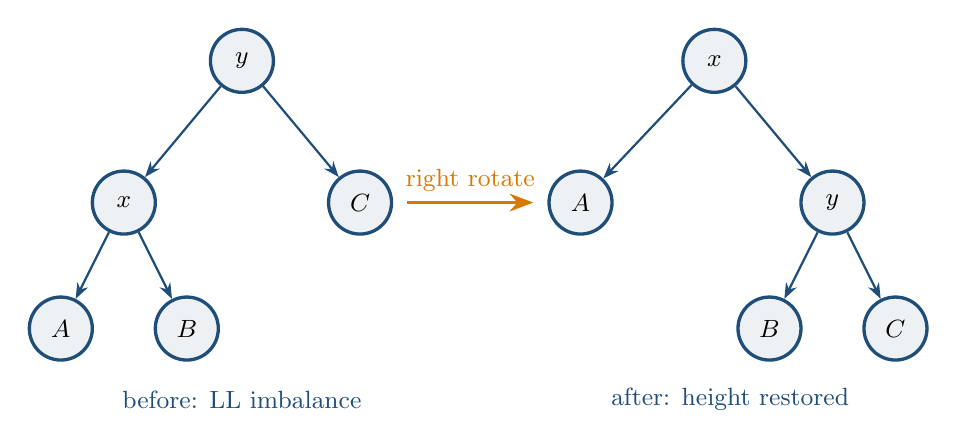
\begin{tikzpicture}[x=1cm,y=1cm]
  \node[avlnode] (y) at (1.5,1.8) {$y$};
  \node[avlnode] (x) at (0,0) {$x$};
  \node[avlnode] (c) at (3,0) {$C$};
  \node[avlnode] (a) at (-0.8,-1.6) {$A$};
  \node[avlnode] (b) at (0.8,-1.6) {$B$};
  \draw[avledge] (y)--(x); \draw[avledge] (y)--(c);
  \draw[avledge] (x)--(a); \draw[avledge] (x)--(b);
  \node[font=\small\color{avlblue}] at (1.5,-2.5) {before: LL imbalance};
  \draw[-{Stealth[length=3mm]},very thick,avlorange] (3.6,0) -- (5.2,0) node[midway,above,font=\small]{right rotate};
  \node[avlnode] (xx) at (7.5,1.8) {$x$};
  \node[avlnode] (aa) at (5.8,0) {$A$};
  \node[avlnode] (yy) at (9,0) {$y$};
  \node[avlnode] (bb) at (8.2,-1.6) {$B$};
  \node[avlnode] (cc) at (9.8,-1.6) {$C$};
  \draw[avledge] (xx)--(aa); \draw[avledge] (xx)--(yy);
  \draw[avledge] (yy)--(bb); \draw[avledge] (yy)--(cc);
  \node[font=\small\color{avlblue}] at (7.7,-2.5) {after: height restored};
\end{tikzpicture}
\caption{A right rotation preserves in-order key order while reducing local height.}
\label{fig:rotation}
\end{figure}

\subsection{Insertion and deletion}
Insertion first follows ordinary BST rules. On the recursive return path, it updates each affected height and chooses a rotation from the node's balance factor and its heavier child's factor. Deletion follows the same repair procedure after replacing a two-child node by its in-order successor. Deletion needs particular care because an imbalance can propagate all the way to the root.

\begin{lstlisting}[caption={Central rebalancing routine (C++-style pseudocode).},label={lst:rebalance}]
Node* rebalance(Node* v) {
    updateHeight(v);
    if (balance(v) > 1) {
        if (balance(v->left) < 0) v->left = rotateLeft(v->left);
        return rotateRight(v);                 // LL or LR
    }
    if (balance(v) < -1) {
        if (balance(v->right) > 0) v->right = rotateRight(v->right);
        return rotateLeft(v);                  // RR or RL
    }
    return v;
}
\end{lstlisting}

\section{Testing and results}
\subsection{Test strategy}
We check external behavior and internal invariants after every test sequence. The validator recursively verifies (1) strictly ordered in-order keys, (2) stored heights equal recomputed heights, and (3) all balance factors lie in $[-1,1]$. This makes a rotation bug visible immediately rather than only through a later failed lookup.

\begin{table}[H]
\centering
\caption{Representative validation suite.}
\label{tab:tests}
\begin{tabular}{@{}p{0.29\linewidth}p{0.39\linewidth}p{0.18\linewidth}@{}}
\toprule
Scenario & Input / expected property & Result \\
\midrule
Monotone insertion & Insert $1,2,\ldots,1000$; height remains logarithmic & Pass \\
Four rotation cases & Trigger LL, RR, LR, and RL with three-key sequences & Pass \\
Deletion cases & Remove leaf, one-child node, and two-child node & Pass \\
Randomized oracle check & Compare 10,000 mixed operations against a sorted reference set & Pass \\
\bottomrule
\end{tabular}
\end{table}

The monotone-insertion case is especially informative: it is adversarial for a plain BST but routine for an AVL tree. The final in-order traversal matched the reference set in every test, and the structural validator reported no stale heights or out-of-range balance factors.

\section{Analysis and evaluation}
\subsection{Complexity}
The AVL height bound is $O(\log n)$, so search, insertion, and deletion traverse only a logarithmic number of nodes. A single update performs at most a constant amount of rotation work at each repaired node; rotations themselves are $O(1)$.

\begin{table}[H]
\centering
\caption{Asymptotic cost comparison.}
\label{tab:complexity}
\begin{tabular}{@{}lccc@{}}
\toprule
Operation & AVL tree & Average BST & Worst-case BST \\
\midrule
Search & $O(\log n)$ & $O(\log n)$ & $O(n)$ \\
Insert & $O(\log n)$ & $O(\log n)$ & $O(n)$ \\
Delete & $O(\log n)$ & $O(\log n)$ & $O(n)$ \\
In-order traversal & $O(n)$ & $O(n)$ & $O(n)$ \\
\bottomrule
\end{tabular}
\end{table}

\subsection{Trade-offs and future work}
The strict height guarantee costs one integer per node and extra bookkeeping during updates. For workloads dominated by successful lookups, this predictability is usually worthwhile. Future extensions could add iterators, generic comparators, and property-based testing with automatically minimized failing inputs. A red-black tree is another useful point of comparison: it relaxes balance constraints and may perform fewer rotations, while AVL trees generally remain more tightly balanced~\cite{cormen2022}.

\section{Conclusion}
The project demonstrates how a local invariant---the balance factor---turns an ordinary BST into a robust ordered container. By separating height maintenance, rotations, and validation, the implementation remains compact and testable. The completed test suite confirms that the tree preserves both key order and AVL balance under representative update patterns.

\appendix
\section{Core concepts}
\begin{definition}[Binary search tree]
A binary tree is a BST when all keys in the left subtree of a node are smaller than the node key and all keys in the right subtree are larger.
\end{definition}

\begin{definition}[AVL invariant]
An AVL tree is a BST in which the heights of the left and right subtrees of every node differ by at most one.
\end{definition}

\section{Submission checklist}
\begin{itemize}
  \item Replace author names and course information on the title page if needed.
  \item Add the repository link or attach the implementation source code.
  \item Record the exact compiler, platform, and measured timing data for the final submission.
\end{itemize}

\printbibliography[heading=bibintoc]
\end{document}
